\ifdefined\MAINDOC\else
\documentclass[10pt, a4paper, fleqn]{article}
\usepackage{base}

\begin{document}
    \title{Skript Mathe 2}
    \date{20. Juni 2018}
    \maketitle
\fi

\subsection{Beispiele}
\begin{enumerate}[a)]
    \item Für $f(x) = x^n$ ist $f^{-1} (y) = \sqrt[n]{y}$ \\
    $\imp$ Ableitung von $f^{-1}$ wird in $y = f(0) = 0$ unendlich
    groß, da $f'(0) = 0$
    \[
        (f^{-1}(y))' = \frac{1}{n(\sqrt[n]{y})^{n+1}} = \frac{1}{n\sqrt{y^{n-1}}}
        \quad \text{Für $y \neq 0$}
    \]
    \begin{minipage}{0.6\textwidth}
        \item $\sin: (-\frac{\pi}{2}, \frac{\pi}{2}) \to (-1, 1)$
        
        Sei $y = \sin x, \ y \in (-1, 1)$
        \[
            \arcsin' y = \frac{1}{\cos x} = \frac{1}{\sqrt{1 - \sin^2 x}} =
            \frac{1}{\sqrt{1 - y^2}}
        \]
    \end{minipage}
    \begin{minipage}{0.4\textwidth}
        \begin{tikzpicture}
            \begin{axis}[
                width = \textwidth,
                axis x line = center,
                axis y line = center,
                ytick = \empty,
                xtick = {-90, 90},
                xticklabels = {$-\dfrac{\pi}{2}$, $\dfrac{\pi}{2}$},
                domain = -100:100
            ]
            \addplot[color = black] {sin(x)};
            \end{axis}
        \end{tikzpicture}
    \end{minipage}
    Analog:
    \[\begin{aligned}
        &\bullet& \arccos' y &= \dfrac{1}{\sqrt{1-y^2}} &&y \in (-1, 1) \\
        &\bullet& \arctan' y &= \dfrac{1}{1 + y^2} &&y \in \IR \\
        &\bullet& \arccotan' y &= \dfrac{1}{1 + y^2} &&y \in \IR
    \end{aligned}\]
    
    \item 
    \abovedisplayskip = -\baselineskip % TODO Use this in other places, works really well!
    \[\begin{aligned}
        f &: \IR \to \IR_{> 0} &&f(x) = e^x \\
        f^{-1} &: \IR \to \IR  &&f(y) = \ln y
    \end{aligned}\]
    \[\imp \ln' y = \frac{1}{e^{\ln y}} = \frac{1}{y}\]
    \[\begin{aligned}
        \imp \ln(|y|)' &= \begin{cases}
            \frac{1}{y} & y > 0 \\
            (-1) \cdot \frac{1}{-y} & y < 0 \text{ (Kettenregel)}
        \end{cases} \\
        &= \frac{1}{y} \text{ für } y \neq 0
    \end{aligned}\]
\end{enumerate}

\subsection{Logarithmische Ableitung}
Für $f: \IR \to \IR \setminus \{0\}, f$ differenzierbar, ist
\[
    (\ln |f(x)|)' = \frac{f'(x)}{f(x)} \quad \text{(6.14c + Kettenregel)}
\]
\textbf{Beispiel: } $f'(x) = e^x \cdot (\sin x + 2) \cdot x^5 \quad x \neq 0 \imp f(x) \neq 0$
\[\begin{aligned}
    &\ln(|f(x)|) = x + \ln(\sin x + 2) + 5 \cdot \ln |x| \\
    &\imp (\ln|f(x)|)' = 1 + \frac{\cos x}{\sin x + 2} + \frac{5}{x} = \frac{f'(x)}{f(x)} \\
    &\imp f'(x) = \qt{1 + \frac{\cos x}{\sin x + 2} + \frac{5}{x}}(e^x(\sin x + 2) x^5) \\
    &= x^4 e^x(x(\sin x + 2)) + x \cdot \cos x + 5 \sin(x + 2) \text{ für } x \neq 0
\end{aligned}\]

\textbf{Bemerkung: }

Man kann zeigen, dass die Ableitung auch auf Funktionen mit Werten in ganz $\IR$
anwendbar ist. Dazu bildet man die stetige Fortsetzung von \\ $f'(x)$ auf $\{x \ | \ f(x) = 0\}$

$\imp$ Beispiel gilt auch für $x = 0$. Dann ist $f'(0) = 0$.

\subsection{Satz: Ableitung elementarer Funktionen}
\begin{itemize}
    \item $(a^x)' = (\ln a) \cdot a^x, a > 0, x \in \IR$
    \item $(x^\alpha)' = \alpha x^{\alpha - 1}, \alpha \in \IR, x > 0$
    \item $(x^x)' = (\ln x + 1) \cdot x^x, x > 0$
\end{itemize}

\textbf{Beweis: }
\[
    (a^x)' = (e^{\ln(a^x)})' = (e^{x \cdot \ln a})' =
    \underset{\mathclap{\text{innere $\cdot$ äußere Ableitung}}}{(\ln a) \cdot (e^{x \cdot \ln(a)})} =
    (\ln a) \cdot a^x 
\]
Rest analog $\qed$

\section*{Kurvendiskussion}
\subsection{Definition: Extremum}

$f: D \to \IR$ besitzt in $x_0 \in D$ ein lokales $\underbrace{\text{Maxmimum (Minimum)}}_{\text{Extremum}}$, \\
wenn es ein Intervall $U = (x_0 - \delta, x_0 + \delta) \subseteq D, \delta > 0$ gibt, so dass

$f(x_0) \underset{\hbox{$(\leq)$}}{\geq} f(x) \quad \forall x \in U$ ($\leftarrow$ Umgebung von $x$)

$f$ besitzt in $x_0 \in D$ ein globales Maxmimum (Minimum),

wenn $f(x_0) \underset{\hbox{$(\leq)$}}{\geq} f(x) \quad \forall x \in D$

\subsection{Notwendige Bedingung für lokale Extrema}
Sei $f: D \to \IR$ differenzierbar in $x_0 \in D$.
Falls $f$ in $x_0$ ein lokales Extremum besitzt, so ist $f'(x_0) = 0$.
\bigskip

\begin{minipage}{0.5\textwidth}
    \begin{center}
        \begin{tikzpicture}
            \begin{axis}[
                width = 0.8\textwidth,
                axis lines* = center,
                ytick = \empty,
                xtick = \empty,
            ]
            \addplot[color = black] {-x^2};
            \draw (0, 0) node[circle, fill = black, scale = 0.3]{};
            \end{axis}
        \end{tikzpicture}

        Differenzierbar  
    \end{center}
\end{minipage}
\begin{minipage}{0.5\textwidth}
    \begin{center}
        \begin{tikzpicture}
            \begin{axis}[
                width = 0.8\textwidth,
                axis y line* = center,
                axis x line = none,
                ytick = \empty,
                xtick = \empty,
            ]
            \addplot[color = black] {-abs(x)};
            \draw (0, 0) node[circle, fill = black, scale = 0.3]{};
            \end{axis}
        \end{tikzpicture}

        Nicht differenzierbar
    \end{center}
\end{minipage}
\bigskip

\textbf{Beweis: } Sei $U = (x_0 - \delta , x_0 + \delta), \delta > 0$ und

$\underbrace{f(x_0) \geq f(x)}_{\text{Maxmimum}} \quad \forall x \in U$.
\begin{itemize}
    \item $f(x_0) \geq f(x_0 + h) \quad \forall h < s$.
    \item $f$ differenzierbar $\imp f'(x_0) = \lim\limits_{h \to 0} \dfrac{f(x_0 + h) - f(x_0)}{h}$
    \[\begin{aligned}
        &\imp \lim_{h \to 0^+} \frac{\overbrace{f(x_0 + h) - f(x_0)}^{\leq 0}}{\boxed{h} > 0} \leq 0 \text{ und } \\
        &\lim_{h \to 0^-} \frac{\overbrace{f(x_0 + h) - f(x_0)}^{\leq 0}}{\boxed{h} < 0} \geq 0 \imp f'(x_0) = 0
    \end{aligned}\]
    Für Minimum Analog $\qed$
\end{itemize}
\subsection{Anmerkung}
$f'(x_0) = 0$ ist notwendige Bedingung aber keine hinreichende Bedingung.

\textbf{Beispiel: }
$f(x) = x^3$ hat in $x = 0$ einen Sattelpunkt mit Steigung $0$.
\bigskip

\begin{minipage}{0.4\textwidth}
    \begin{tikzpicture}
        \begin{axis}[
            width = \textwidth,
            axis lines = center,
            ytick = \empty,
            xtick = \empty,
        ]
        \addplot[color = black] {x^3};
        \end{axis}
    \end{tikzpicture}  
\end{minipage}
\begin{minipage}{0.5\textwidth}
    $f$ hat lokales Extremum $\overset{\hbox{$\cancel{\Leftarrow}$}}{\imp} f'(x_0) = 0$
\end{minipage}

\subsection{Mittelwertsätze, Satz von Rolle (1652--1719)}
\begin{enumerate}[1.]
    \item \text{}\\
    \begin{tikzpicture}[
        declare function = {
            f(\x) = \x * 0.6;
            t(\x) = f(\x) - 3;
        }
    ]
        \begin{axis}[
            unit vector ratio* = 1 1 1, 
            xmin = 0, xmax = 14,
            ymin = -1, ymax = 10,
            axis lines = left,
            xtick = {4, 8, 12},
            xticklabels = {$a$, $\xi$, $b$},
            ytick = {2.4, 7.2},
            yticklabels = {$f(a)$, $f(b)$},
            domain = 0:14,
        ]
        \addplot[color = blue, samples = 2] {t(x)};
        \addplot[color = green!60!black, samples = 2] {f(x)};
        \draw[color = red] plot [smooth, tension = 1] coordinates { 
            (4, {f(4)}) (5.5, 6) (8, {t(8)}) (10, 8) (12, {f(12)})
        };
        \addplot[only marks, mark options = {scale = 0.7}] coordinates {
            (4, {f(4)}) (8, {t(8)}) (12, {f(12)})
        };
        \draw[dashed] (4, -1) -- (4, {f(4)}) -- (0, {f(4)});
        \draw[dashed] (12, -1) -- (12, {f(12)}) -- (0, {f(12)});
        \draw[dashed] (8, -1) -- (8, {t(8)});
        \end{axis}
        \draw (7.7, 3.2) node {Tangente};
    \end{tikzpicture}

    \item \text{}\\
    \hspace*{23pt}
    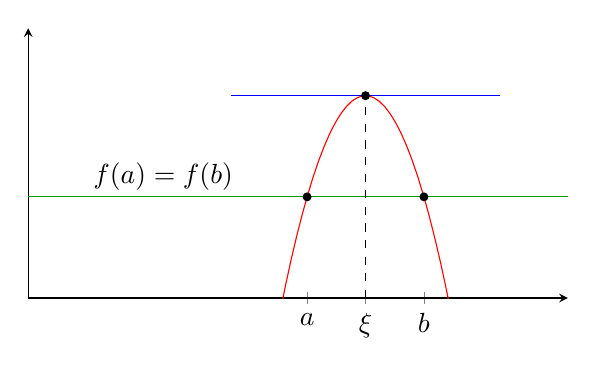
\begin{tikzpicture}[
        declare function = {
            f(\x) = -x^2;
        }
    ]
        \begin{axis}[
            unit vector ratio* = 1 1 1,
            axis lines = left,
            ymin = -6, ymax = 2,
            xtick = {-1.73205080757, 0, 1.73205080757},
            xticklabels = {$a$, $\xi$, $b$},
            ytick = \empty,
            domain = -10:6
        ]
        \addplot[color = red, samples = 50, domain = -4:4] {f(x)};
        \addplot[color = green!60!black, samples = 2] {-3};
        \addplot[color = blue, samples = 2, domain = -4:4] {0};

        \addplot[only marks, mark options = {scale = 0.7}] coordinates {
            ({sqrt(3)}, -3) ({-sqrt(3)}, -3) (0, 0)
        };
        \draw[dashed] (0, -6) -- (0, 0);
        \draw (-6, -2.4) node {$f(a) = f(b)$};
        \end{axis}
    \end{tikzpicture}
\end{enumerate}
Seien $f, g: [a, b] \to \IR$

stetig und differenzierbar in $(a, b), \ g'(x) \neq 0 \quad \forall x \in (a, b)$
\begin{enumerate}[1.]
    \item
    $\imp \exists \xi \in (a, b): \dfrac{f(b) - f(a)}{b - a} = f'(\xi)$

    1. Mittelwertsatz

    \item
    $f(a) = f(b) \imp \exists \xi \in (a, b): f'(\xi) = 0$

    Satz von Rolle

    \item
    $\exists \xi \in (a,b): \dfrac{f(b) - f(a)}{g(b) - g(a)} = \dfrac{f'(\xi)}{g'(\xi)}$

    2. Mittelwertsatz
\end{enumerate}
\textbf{Beweis: }
\begin{enumerate}
    \item [2.] $f$ stetig in $[a, b]$

    $\underset{3.36}{\imp} f$ besitzt Maxmimum $M$ und Minimum $m$ in $[a, b]$.

    D.h: $m \leq f(x) \leq M \quad \forall x \in [a, b]$
\end{enumerate}
\ifdefined\MAINDOC\else
\end{document}
\fi